\newpage
\section{Thermal cycling of detector electronics}
\label{thermal_cycling}
Operating temperatures inside the \gls{STS} enclosure are dictated by the total non-ionizing dose and noise levels. The temperature conditions in the STS could have repercussions on the functioning of detector electronics. Nevertheless, for the first few years of operation, the ambient temperatures will be higher than \SI{-10}{\celsius}. Operating scenarios of the \gls{STS} together with other constraints related to, for example, the soft errors rate in the low voltage powering of the \gls{FEE}, define the testing procedures for all the electronics which will experience thermally induced mechanical stresses.

One of the elements of the detector module which can experience significant mechanical stresses is the \gls{FEB}.
During the commissioning and operation, the \glspl{FEB} will experience many power cycles. As reported in the~\cite{CBM_PR_2021}, the power cycling of the \glspl{FEB} at room temperature of about \SI{20}{\celsius} run flawlessly, not identifying any issues with the boards. Nevertheless, the testing did not reproduce the STS operational conditions.

To evaluate the behavior of the board in realistic conditions, a thermal cycling setup was envisioned. Thermal cycling testing is usually performed in order to determine the ability of different components and solder interconnects to resist extreme temperature changes. Permanent changes to the electrical or physical features may compromise the detector modules performance.

 For the control and monitoring of devices, as well as for the processing of data the previously developed control framework was introduced. Implementation of the EPICS-based framework played a crucial role, as it enabled live monitoring of many parameters during the tests.

\subsection{Nominal operation scenario of the STS}
\label{nominal}

In the nominal operation scenario at the end of the STS lifetime, the \glspl{FEB} are operated at the nominal power ($\approx8\,W$), and any excess heat is evacuated by cooling liquid (NOVEC 649) flowing through the \gls{FEB} cooling plate at \SI{-40}{\celsius}. Figure~\ref{fig_coolinkg_block_nominal} and~\ref{fig_nominal_febs}, depict thermal simulations of the cooling plate, \gls{FEB} box, and the \gls{FEB} for the nominal operation scenario.

During periods in which the temperature will change due to transitions between detector states, the electronics will experience thermal stresses, which will partially occur with the electronics switched on. The cases discussed relate to the worst-case scenarios, in which the temperature differences are the highest. 
    
\begin{figure}[!h]
\centering
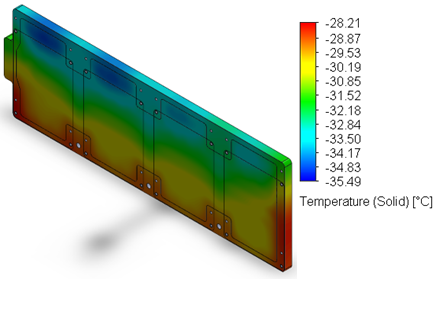
\includegraphics[width=0.6\columnwidth]{Chapter4/images/cooling_block_nominal.png}
\caption{Temperature distribution on the cooling plate for the nominal operation scenario~\cite{Agarwal}.}
\label{fig_coolinkg_block_nominal}
\end{figure}

\newpage

\begin{figure}[!h]
\centering
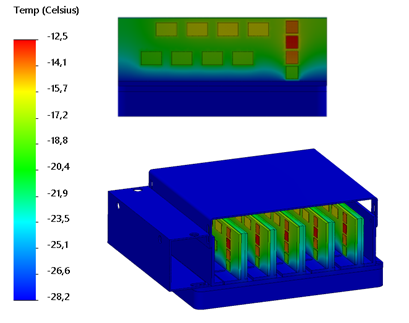
\includegraphics[width=0.62\columnwidth]{Chapter4/images/nominal_febs.png}
\caption{Temperature distribution in the \gls{FEB} box containting 10 \glspl{FEB} (bottom of the figure) and on the \gls{FEB} for the nominal operation scenario (top of the figure)~\cite{Agarwal}. }
\label{fig_nominal_febs}
\end{figure}


During the active, nominal phase of operation, the temperature change of the electronics could be $\Delta T \approx \SI{20}{\celsius}$. On the other hand, simulations from Figure~\ref{fig_nominal_febs} indicate the minimum temperature the electronics will reach during the operation. This operation mode is summarized in Figure~\ref{fig_nominal_scenario}.  The difference is associated with a slow increase of the coolant temperature from \SI{-40}{\celsius} to \SI{-20}{\celsius}. After switching off the electronics, the temperature reaches the temperature of the cooling plate. The change will be $\Delta T \approx \SI{20}{\celsius}$ (from e.g., \SI{0}{\celsius} to \SI{-20}{\celsius}). These temperatures provide an indication of minimum and maximum thermal cycling set points.  

\begin{figure}[!h]
\centering
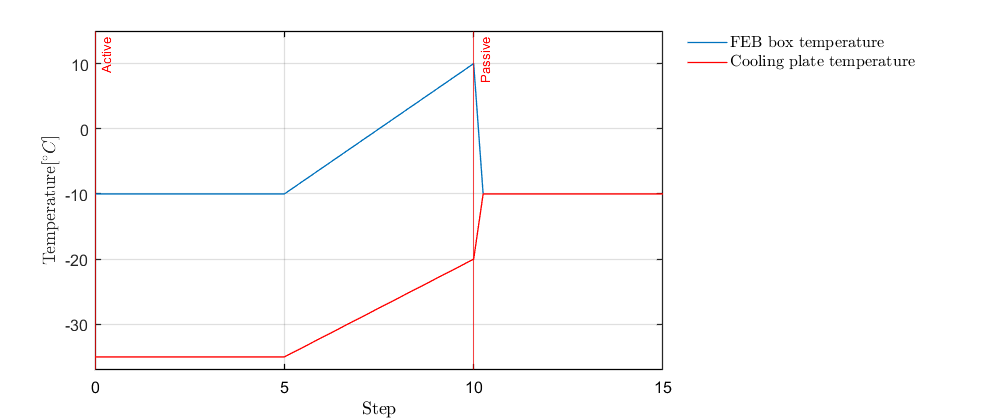
\includegraphics[width=0.85\columnwidth]{Chapter4/images/nominal_all.png}
\caption{An example of \gls{STS} state transition from operation to safe state - comparison of temperatures of a \gls{FEB} box and cooling liquid temperature. A step could be defined as a generic time period.}
\label{fig_nominal_scenario}
\end{figure}


\subsection{Partial shutdown scenario of the STS}
\label{reboot}

At any given point during operation, the operator may need to power cycle a \gls{FEB}(s). In this scenario, the temperature of a given \gls{FEB} may change drastically due to the temporary loss of power. The amount of the thermally induced mechanical stress depends on reboot and configuration time. Besides, in case of a radiation-induced soft error in the power supply, the downtime of a \gls{FEB} may be difficult to predict. If the soft error is instantly recoverable, the FEB will be powered on in seconds after switching off, limiting a deteriorating effect of large temperature changes $\Delta T$.

Figure~\ref{fig_reboot_box} depicts the scenario in which only 5 out of 10 \glspl{FEB} are on, which results in effectively lower temperatures in comparison to the nominal scenario. Nevertheless, the $\Delta T$ remains the same as in the nominal operation scenario. During the operation, this scenario will probably last for a short time (range of seconds), and the temperature of the rebooted \gls{FEB} will not reach as low temperatures as depicted in the previous simulations.


%\begin{figure}[!h]
%\centering
%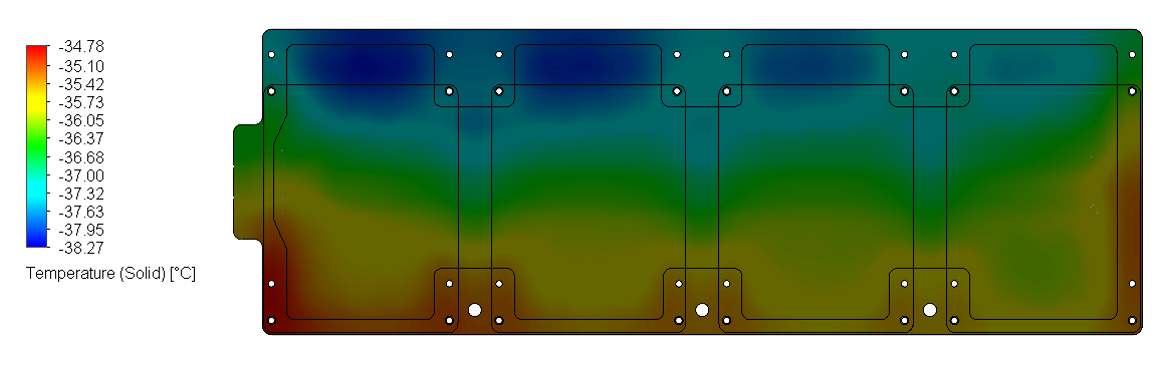
\includegraphics[width=0.85\columnwidth]{Chapter4/images/reboot_cooling_plate.png}
%\caption{Temperature distribution on the cooling plate for the reboot scenario}
%\label{fig_reboot_scenario}
%\end{figure}

\begin{figure}[!h]
\centering
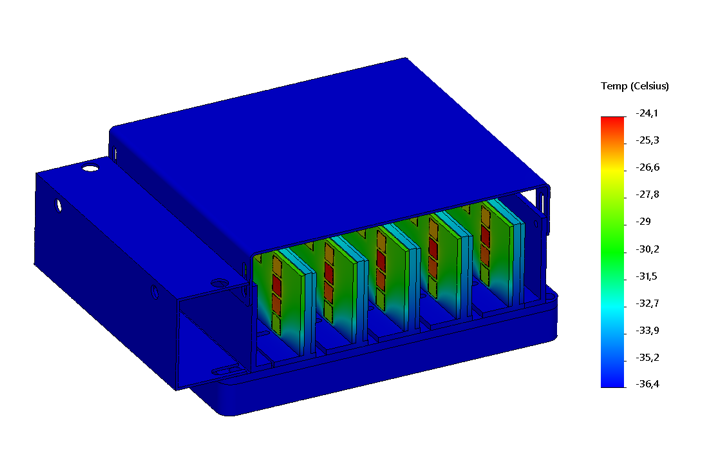
\includegraphics[width=0.57\columnwidth]{Chapter4/images/reboot_box.png}
\caption{Temperature distribution for the partially unpowered \gls{FEB}~\cite{Agarwal}. Each cooling shelf inside the \gls{FEB} box has two glued boards, and one of them is powered.}
\label{fig_reboot_box}
\end{figure}

\begin{figure}[!h]
\centering
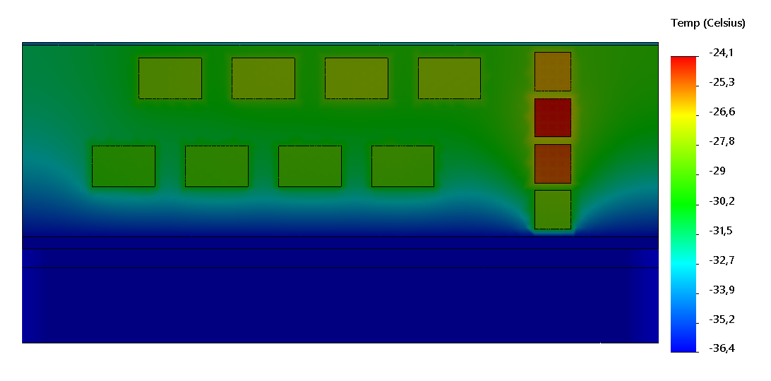
\includegraphics[width=0.6\columnwidth]{Chapter4/images/reboot_FEB.png}
\caption{Temperature distribution of a \gls{FEB} for the partial shutdown scenario~\cite{Agarwal}.}
\label{fig_reboot_FEB}
\end{figure}

\begin{figure}[!h]
\centering
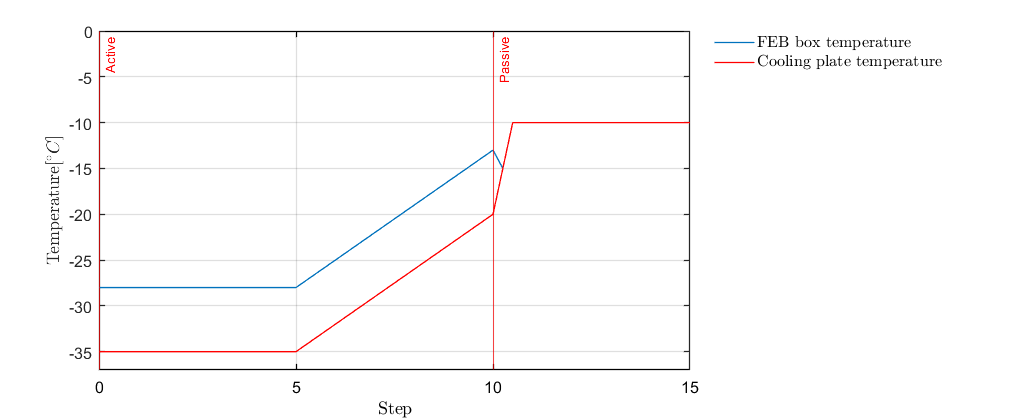
\includegraphics[width=0.85\columnwidth]{Chapter4/images/nominal.png}
\caption{An example of \gls{STS} state transition from operation to safe state - comparison of temperatures of a \gls{FEB} box and cooling liquid temperature. Step represent a generic time period, indicating the rate of changes in the detector.}
\label{fig_reboot_nominal2}
\end{figure}

\subsection{Loss of power scenario of the STS}
\label{power_loss}
The last considered scenario is the so-called loss of power scenario. Out of the three introduced scenarios, it is the least probable one, but it also leads to significant data loss, as 10 \glspl{FEB} would stop sending data. Such a scenario could happen if all the connected low-voltage channels switch off, e.g., due to radiation. In this case, the \glspl{FEB} would reach the temperature of the cooling block ($T \approx \SI{-40}{\celsius}$) if the powering was not turned on within seconds.

\subsection{Influence of the coefficient of thermal expansion on the PCB performance}

The coefficient of thermal expansion (\gls{CTE}) is an important property of materials that affects relative movement between \gls{PCB} components. \gls{CTE} should be a concern when it comes to \glspl{PCB}, as out-of-plane \gls{CTE} could cause cracking and delamination, while in-plane \gls{CTE} may cause for example shear failures in solder joints~\cite{cte_report}. The \gls{STS} \gls{FEB} is equipped with many components which could be the reason for malfunctions at low temperatures, making analysis of potential causes a complex task. 
These components can be seen in Figure~\ref{fig_globtop}.
\begin{figure}[!h]
\centering
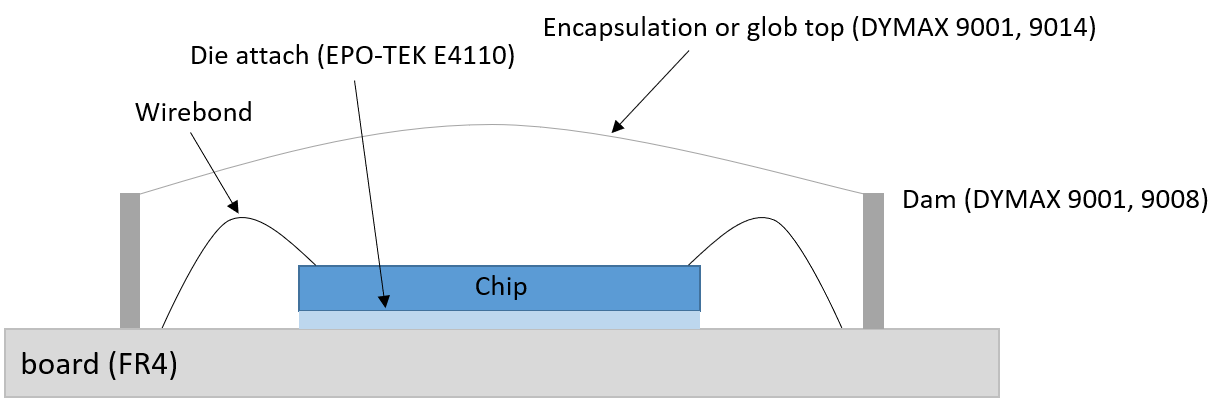
\includegraphics[width=0.85\columnwidth]{Chapter4/images/glob_topped_device.png}
\caption{Schematics of the glob-topped device with the materials used for the thermal cycling of different FEB flavors.}
\label{fig_globtop}
\end{figure}

Both the \gls{LDO} regulators and STS-XYTERs are covered with high viscosity glues which are known as glob top\footnote{protective epoxy-based material for microelectronics}. Apart from \gls{CTE}, the performance of the glob top material depends on many other factors:
\begin{itemize}
    \item adhesion to the substrates,
    \item part geometry (including the mass of the components in contact),
    \item temperature extremes,
    \item number of cycles, and transition times.
\end{itemize}


The most common phenomena which cause damage to the glob-topped device are:
\begin{itemize}
    \item wire-bond failure,
    \item failure of the chip to board or substrate joint,
    \item damage to protective chip passivization layer,
    \item chip cracking,
    \item metallization pattern shift,
    \item development of voids or notches in metallization tracks. 
\end{itemize}


According to the data on electronics failures analyzed by the U.S. Air Force over about 20 years, it was shown that 50\% of these failures are related to connectors, 30\% to interconnects, and 20\% to component
parts. Hardware failures may occur due to handling, vibrations, or stress of different origins (including thermal stress). About 55\% of the electronics failures are due to high temperatures and temperature cycling, 20\% of the failures are related to vibration and shock, and 20\% are due to humidity~\cite{thermal_electronics}. 

To protect the STS microelectronics, DYMAX 9001 was the glob top choice for the \glspl{FEB}, and it was then replaced by its successor DYMAX 9014. The \gls{LDO} regulators and \glspl{ASIC} are made of silicon. The linear CTE of glob top materials (DYMAX 9001, DYMAX 9014, DYMAX 9008) and conductive glue (EPO-TEK E4110) is by an order of magnitude higher than the coefficient for the \glspl{PCB} and silicon. Additionally, a volume expansion influences the relative position of different components during thermal cycling.

\begin{table}[!h]
\begin{center}
\caption{Coefficient of thermal expansion of different materials below the glass transition temperature.}
\begin{tabular}{ll}
\hline
\multicolumn{1}{c}{Material} & \multicolumn{1}{c}{CTE $\alpha_{2}$} [\si{\micro\metre\per\metre\per\celsius]}] \\ \hline
DYMAX 9001-E-V3.5~\cite{9001}            & 180                                  \\
DYMAX 9014~\cite{9014}                   & 192                                  \\
DYMAX 9008~\cite{9008}                   & 230                                  \\
EPO-TEK E4110~\cite{4110}                & 150                                  \\ \hline
FR4 (\gls{PCB} material)~\cite{FR4}                          & 15                                   \\
Silicon~\cite{Si}                           & 2.6                                 
\end{tabular}
\label{TCE}
\end{center}
\end{table}

Three main components which need to be analyzed during the testing are the glues (glob top and conductive glue), bonds, and microelectronics (\gls{LDO} regulator and STS-XYTER). From the thermal cycling point of view, power dissipation is one of the key differences between the DC linear voltage regulator and the front-end chip. Figure~\ref{fig_temperatures_camera} depicts the temperature distribution of a powered board. The board was screwed to the cooling plate, which was at \SI{20}{\celsius}.

\begin{figure}[!h]
\centering
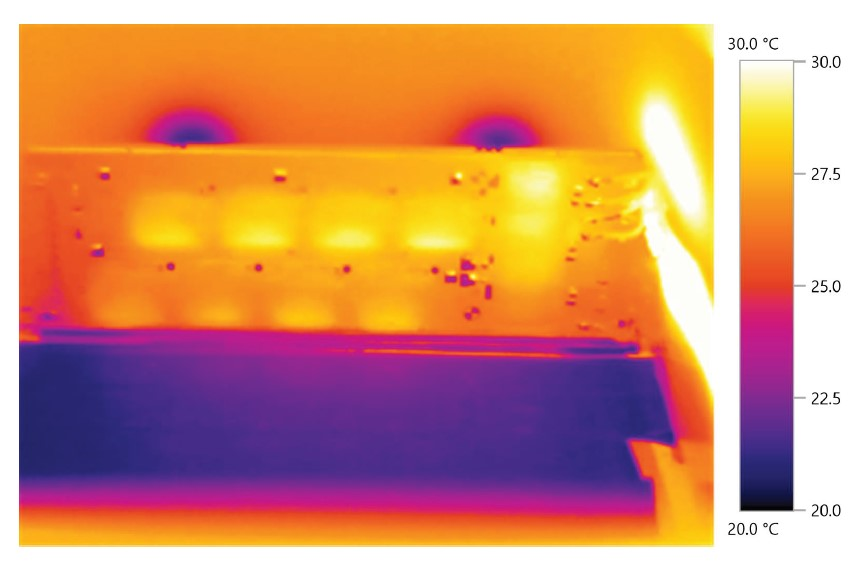
\includegraphics[width=0.6\columnwidth]{Chapter4/images/feb_thermal.jpg}
\caption{Temperature of the \gls{FEB} components measured with a thermal camera for the low power consumption scenario, \cite{leo_electronics}. The \gls{LDO} (on the right side of the picture) appear to be hotter than STS-XYTER chips.}
\label{fig_temperatures_camera}
\end{figure}



%\begin{figure}[!h]
%\centering
%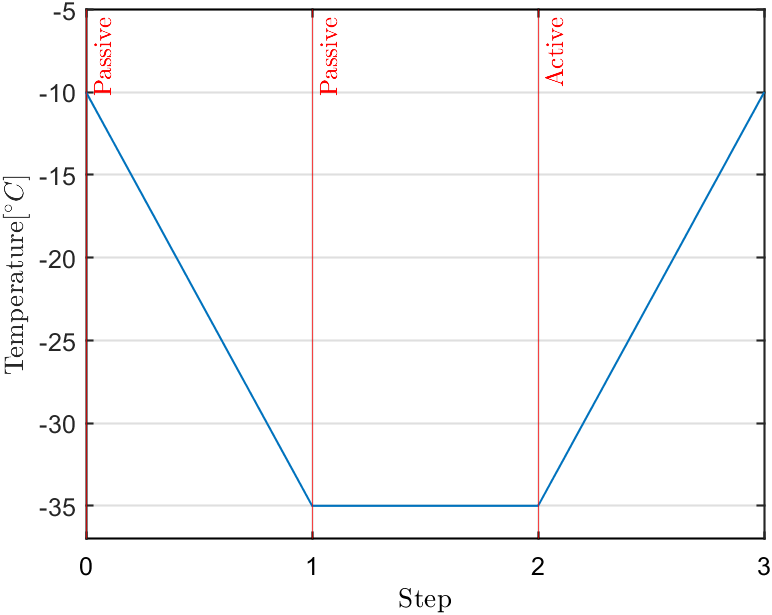
\includegraphics[width=0.55\columnwidth]{Chapter4/images/switchoff.png}
%\caption{Sudden loss of power and bringing the \glspl{FEB} back to operation}
%\label{fig_loss}
%\end{figure}

%\newpage
\subsection{Experimental setup for thermal cycling of STS electronics}
\label{cycling_setup}
In order to investigate the effect of thermal cycles of the FEBs, a setup consisting of FEBs, readout board, Lauda chiller, climatic chamber, temperature sensors and humidity sensors was introduced.
A detailed overview of the setup is depicted in Figure~\ref{fig_setup}. The software part features the Control System Studio (Phoebus) for monitoring, accessing the database (Redis DB), and monitoring the \gls{PV}s. Moreover, all values are saved with archiver appliance. The second node features a LabView-based interface for reading out additional humidity sensors. This node was later on depreciated and relative humidity readouts were taken from the built-in Relative Humidity (\gls{RH}) sensor inside the climatic chamber.

The main objective was thermal cycling of the \glspl{FEB}, which consists of 4 LDO regulators (two 1.2\,V LDO and two 1.8\,V LDO regulators) and 8 \glspl{ASIC}. The diagnostic circuit of the STS-XYTER helped to identify \gls{PCB} related malfunctions. In order to read the temperatures, VDDM, and  \gls{CSA} bias values from the chip, a dedicated soft IOC\footnote{purely software-based \gls{IOC}, not connected to any hardware} was deployed. To acquire the previously mentioned values, the pyEPICS library~\cite{pyEPICS} was used, and the GBTxEMU-based readout chain (see \autoref{tester}) was adjusted to publish the values via channel access protocol. 
\begin{figure}[!h]
\centering
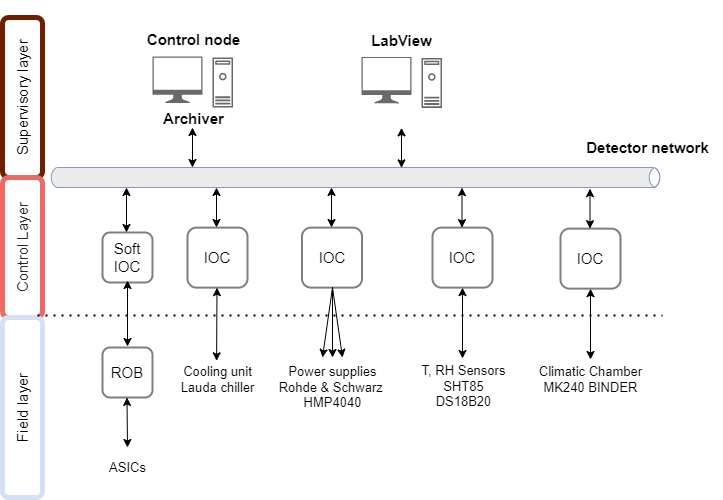
\includegraphics[width=0.85\columnwidth]{Chapter4/images/cycling_scheme.png}
\caption{Schematics of the thermal cycling setup. The readout of relative humidity and temperature sensor is realized through Single Board Microcontrollers~(\gls{SBM}) and Raspberry PI. The python interface was developed for both readout chains (ROB and GBTxEMU based). }
\label{fig_setup}
\end{figure}

\newpage
Apart from the \gls{ASIC}-specific values, are other parameters taken into consideration which are as
follows:
\begin{itemize}
    \item currents and voltages supplied to the 1.2\,V and 1.8\,V \gls{LDO} regulators on the \gls{FEB}, 
    \item temperature changes on the T-shelf (as seen in Figure~\ref{fig_cycling_temps}), which are read-out by a Single Board Microcontroller (\gls{SBM}),
    \item humidity and temperature in the climatic chamber (Sensiron SHT85 sensors plus built-in sensors),
    \item set point temperature of the Kryo 51 coolant (used as an alternative for NOVEC)~\cite{KRYO}.
\end{itemize}

There are different glob-top materials that match the \gls{STS} requirements. To get a better understanding of
their performance, \glspl{FEB} with different glob tops were assembled as shown in Figures 7 and 8. Moreover,
to understand the impact of the glob top material, a board without glob top on \glspl{LDO} regulators was
assembled. In total, four different FEB flavors can be distinguished:
\begin{itemize}
    \item with DYMAX 9001 as the glob top (see Figure~\ref{fig_noglobtop}),
    \item with DYMAX 9014 as the glob top,
    \item with DYMAX 9001 as the fill and DYMAX 9008 as the dam \footnote{Dam and fill is a technique for properly covering wire bonded die. It is a two-step method in which a dam is dispensed around the top of the component first, followed by filling the center.} (see Figure~\ref{fig_cycling_temps}), 
    \item without glob top and \glspl{ASIC} (see Figure~\ref{fig_noglobtop}).
    \end{itemize}
%\newpage
\begin{figure}[!h]
\centering
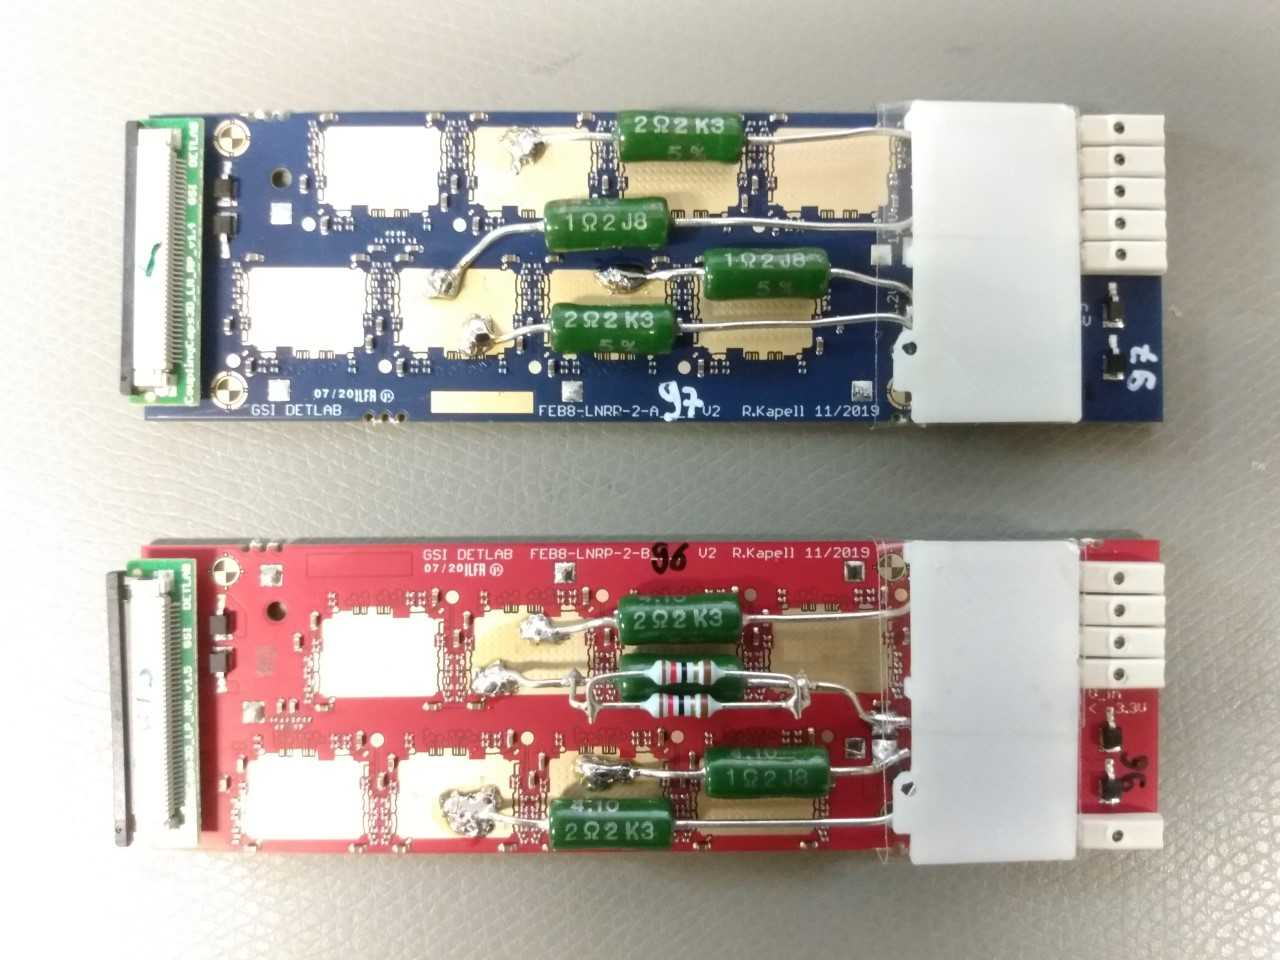
\includegraphics[width=0.45\columnwidth]{Chapter4/images/noglobtop.jpg}
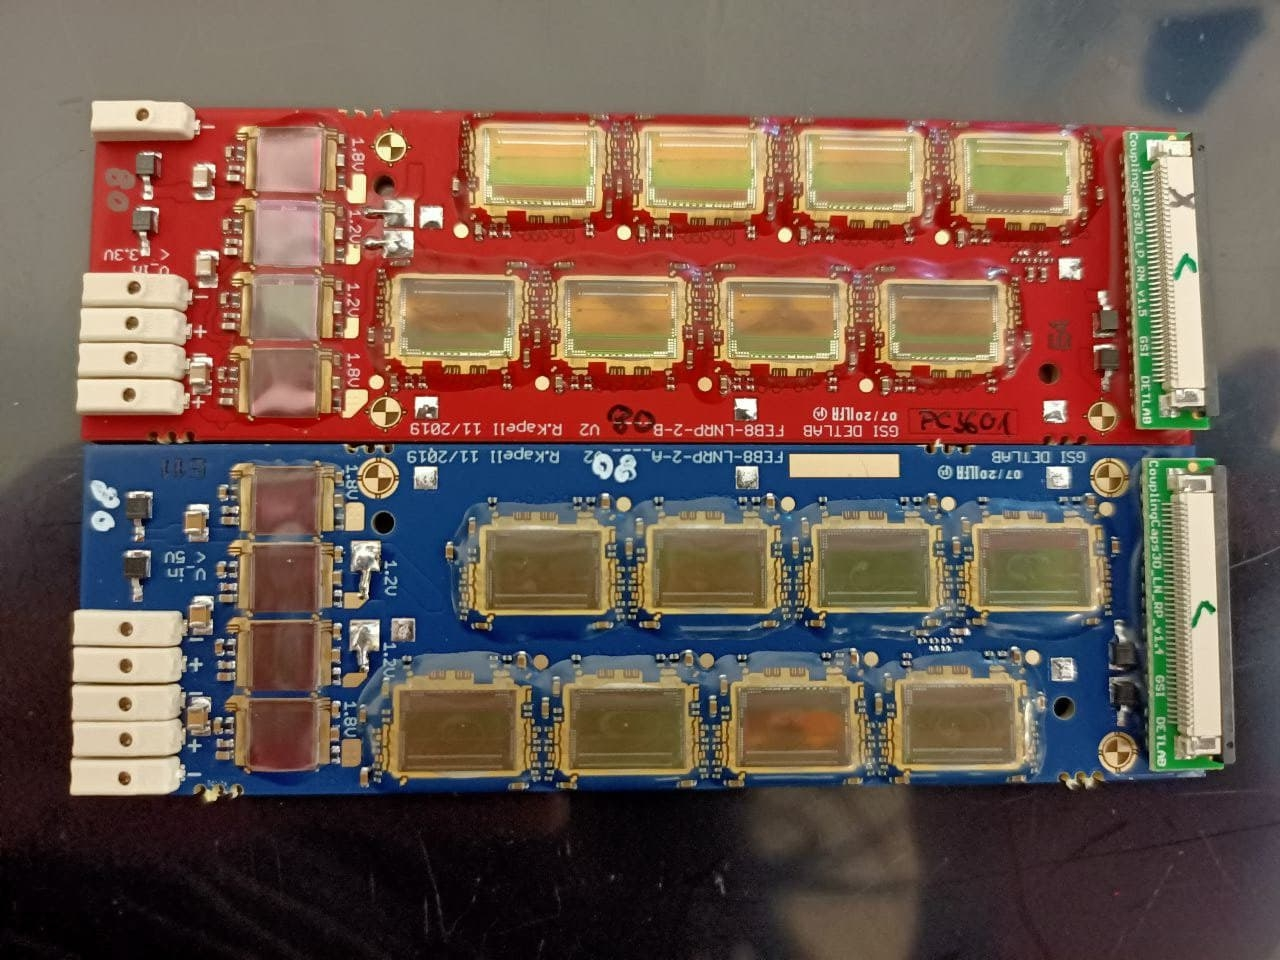
\includegraphics[width=0.45\columnwidth]{Chapter4/images/globtop.jpg}
\caption{The left picture depicts two \glspl{FEB} (version A and B) with the \gls{LDO} regulators covered with 3D-printed protection cap and without glob top. These two boards feature resistors simulating the power consumption of the STS-XYTERs.
The right picture depicts two fully assembled \gls{FEB}s with STS-XYTERS version 2.1 and DYMAX 9001 as the glob top.}
\label{fig_noglobtop}
\end{figure}
\newpage
To prepare for the thermal cycling, the assembled boards (type A and B) were mounted on a cooling shelf (initially with thermal pads, later by gluing it to the T-shelf’s surface) and then eventually placed on a cooling plate in the climatic chamber (see Figure~\ref{fig_cycling_temps}). In order to reproduce similar conditions as in the \gls{STS} (coolant temperature at \SI{-40}{\celsius}) KRYO 51 coolant was used instead of the NOVEC 649 liquid. Additionally, the chamber temperature was always kept below the temperature of the cooling plate to avoid icing. During the cycling, the voltage drop at the \gls{LDO} regulators was the same \SI{0.6}{\volt} for all the boards.

\begin{figure}[!h]
\centering
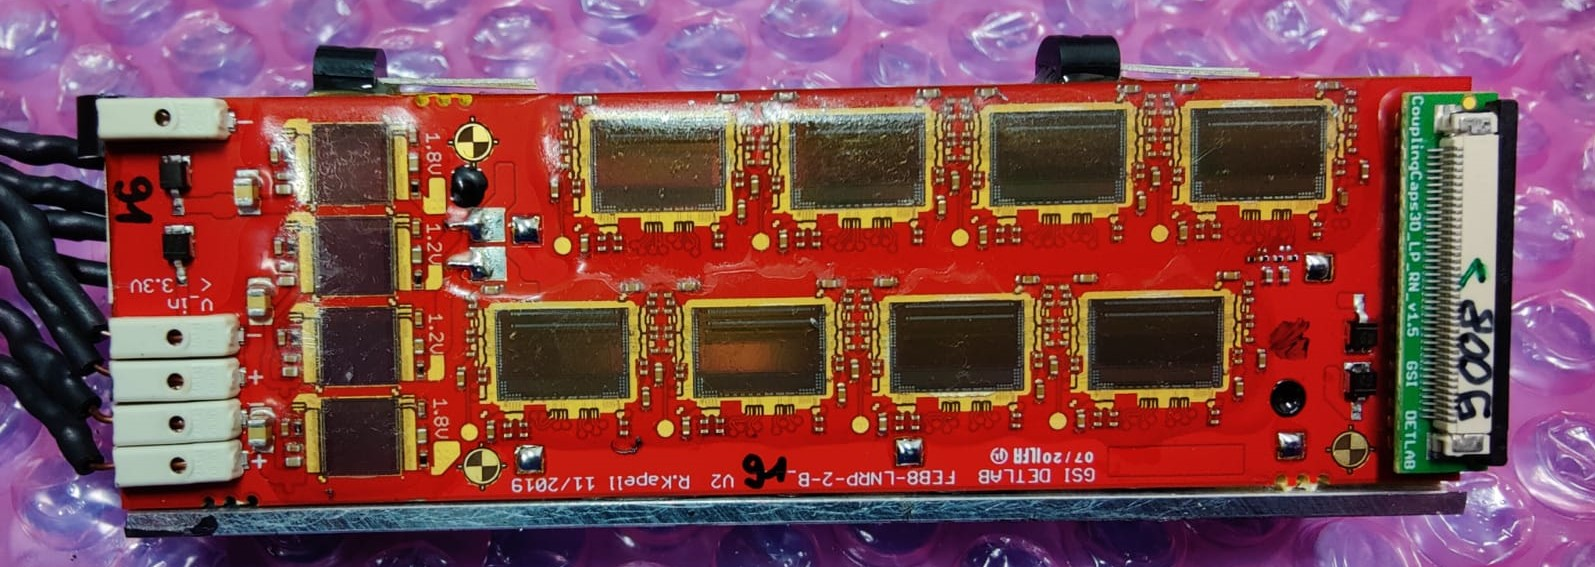
\includegraphics[width=0.5\columnwidth]{Chapter4/images/FEBB_T_sensors.jpeg}
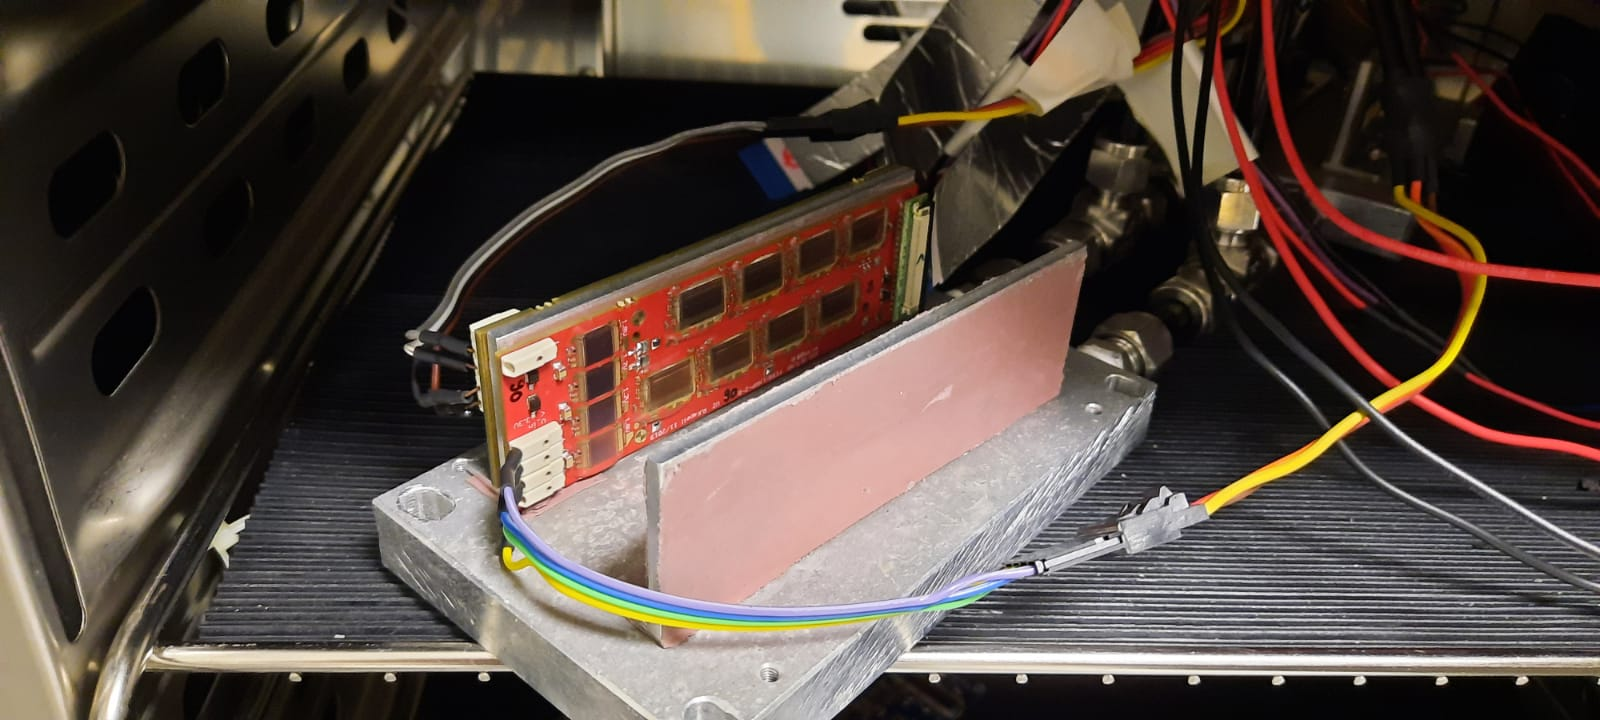
\includegraphics[width=0.4\columnwidth]{Chapter4/images/thermal_setup.jpeg}
\caption{A \gls{FEB} glued to the T-shelf, with 3 DS18B20 temperature sensors installed on the T-shelf (left) and two \gls{FEB}s mounted on a T-shelf with thermal pads inside a climatic chamber (right).}
\label{fig_cycling_temps}
\end{figure}


\subsection{Testing procedure}
The \glspl{FEB}, Readout Boards (\glspl{ROB}), and  Power Boards (\glspl{POB}) are going to be cooled, and they will experience thermal stress on the components. According to the previously introduced operation scenarios, these boards need to withstand:
\begin{itemize}
    \item without the powering $\Delta T\approx\SI{20}{\celsius} $
    \item with powering $\Delta T\approx\SI{20}{\celsius} $
    \item more than 180 cold startups, as indicated in section~\ref{irradiation_results}
\end{itemize}
To find the operational limits of the boards and reproduce the operation scenarios the testing was divided into three stages: passive cycling, active cycling, and power cycles down to \SI{-40}{\celsius} (so-called cold startup). The transition time between the extreme temperatures (for passive and active cycling) is not manually regulated and is solely determined by the power of the Lauda chiller and the climatic chamber.

The main object of the tests was the \gls{FEB}s and its sensitivity to the thermally induced mechanical stresses. In the two main sets of measurements so far, in total 12 \gls{FEB}s in different configurations were tested.  After each round of thermal cycling (usually 50 cycles), the boards were inspected optically under the microscope for any signs of deterioration or visible changes. On the other hand, during the cycling with powering and low-temperature power cycling, the STS-XYTERs were extensively tested. The \glspl{ASIC} test included configuration of the chip, changing \gls{CSA} values to trigger different current consumption, but also ID consistency check, write/read registers test, and internal pulses. By performing the tests, it is possible to evaluate the performance of the board and estimate the influence of the thermal cycling.

\subsubsection{Passive cycling}
Passive cycling refers to a process of changing the temperature of a tested object in a defined range (e.g., from \SI{-20}{\celsius} to \SI{-10}{\celsius}) without powering. This way the stress on the board and its components is lower. Passive cycling was performed in a series of 50 repetitions between optical and electrical inspection. During this part the following temperature differences were tested:
\begin{itemize}
    \item Set A - 8 \glspl{FEB} (3 \glspl{FEB} type A, 3 \glspl{FEB} type B and 2 \glspl{FEB} without glob top and \glspl{ASIC}) were tested in the realistic operating scenarios of the \gls{STS} [\SI{-20}{\celsius}, \SI{-10}{\celsius}], [\SI{-30}{\celsius}, \SI{-10}{\celsius}], [\SI{-40}{\celsius}, \SI{-10}{\celsius}],
    \item Set B 2 out of 4 \glspl{FEB} (1 out of 2 \glspl{FEB} A and 1 out of 2 \glspl{FEB} B) were tested more extensively by increasing $\Delta T$ - [\SI{-20}{\celsius}, \SI{20}{\celsius}].
\end{itemize}
The \glspl{FEB}, regardless of the type (A or B), are treated equally from the mechanical point of view. The components and the way the boards are assembled are the same.


The characteristic of passive cycling was as follows:
\begin{itemize}
    \item  set B was tested without current trip conditions  and for set A the trip current was set to 3.1 A,
    \item the temperature provided by the Lauda chiller was a few degrees higher than the ambient chamber
    temperature, in order to prevent condensation or icing on the electronics,
    \item the periods at the maximum and minimum temperature were always the same and equaled 20 minutes,
\end{itemize}
No performance deterioration was observed during the passive cycling, which is most likely related to the fact that the boards were previously unused. 
%\begin{figure}[!h]
%\centering
%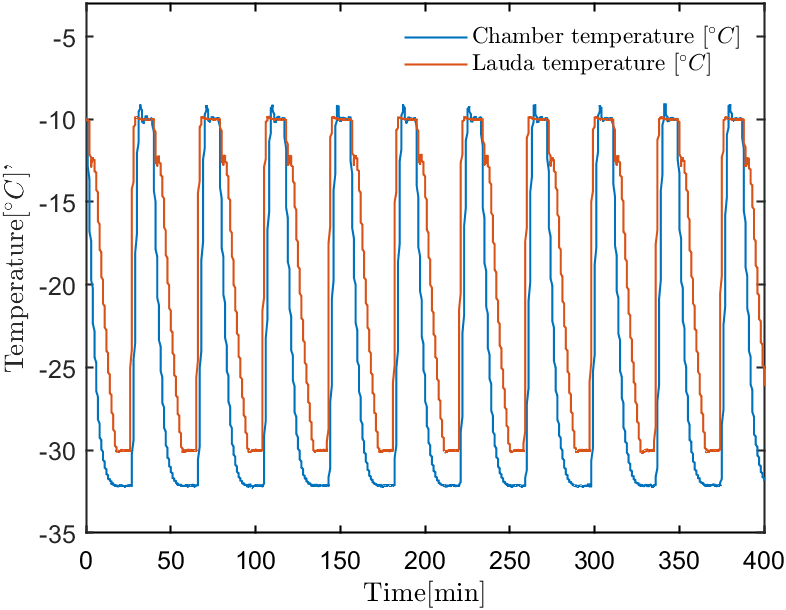
\includegraphics[width=0.55\columnwidth]{Chapter4/images/active_cycling.png}
%\caption{Example of the thermal cycling (passive) of the FEE}
%\label{fig_passive_cycling}
%\end{figure}

\subsubsection{Active cycling}
Active cycling refers to cycling with the electronics switched on at all times. It was performed in a series of 50 repetitions, but due to the fact that the \glspl{FEB} were powered, all the boards and STS-XYTERs were continuously tested, and the current consumed varied by around 1 A at most. The boards underwent the followings cycles:
\begin{itemize}
    \item set A - 8 \glspl{FEB} - [\SI{-10}{\celsius}, \SI{20}{\celsius}] and [\SI{-40}{\celsius}, \SI{-10}{\celsius}],
    \item Set B - 4 \glspl{FEB} (2 \glspl{FEB} A and 2 \glspl{FEB} B)  $\Delta T$ - [\SI{-20}{\celsius}, \SI{20}{\celsius}], [\SI{-30}{\celsius}, \SI{20}{\celsius}], [\SI{-40}{\celsius}, \SI{20}{\celsius}].
\end{itemize}

\begin{figure}[!h]
\centering
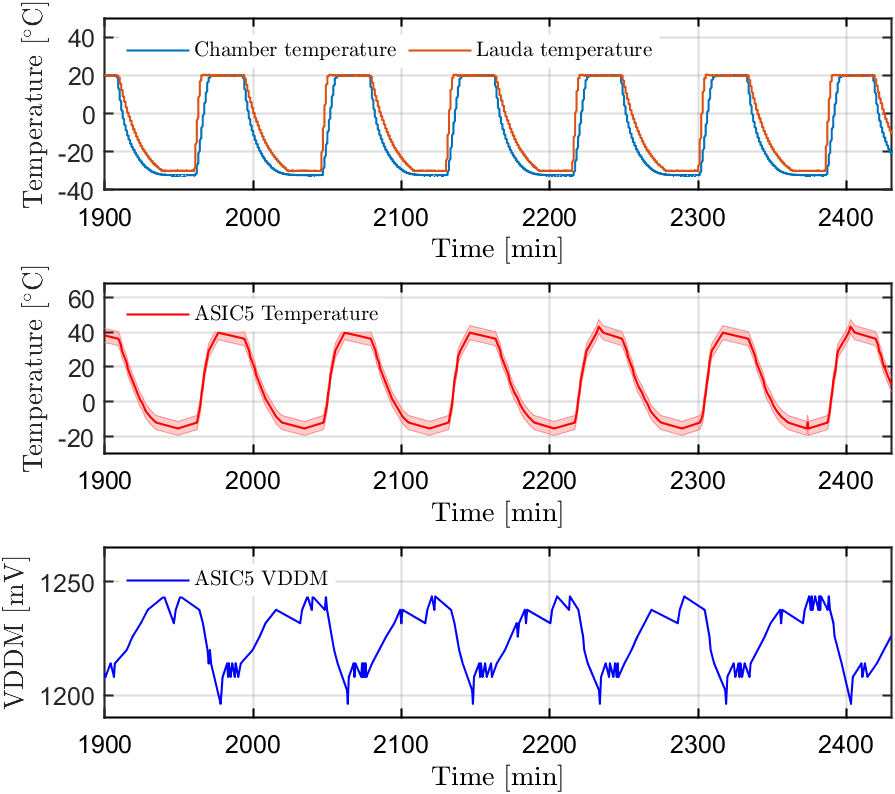
\includegraphics[width=0.65\columnwidth]{Chapter4/images/FEB0ASIC5COMP.png}
\caption{A detailed view on the performed active cycling. The top figure depicts the temperature of the chamber temperature and the set point of the Lauda chiller. Two lower figures show how the readout of temperature and VDDM from a chosen STS-XYTER depends on the cycling temperature. }
\label{fig_active_detailed}
\end{figure}
A detailed view of a few cycles is presented in Figure~\ref{fig_active_detailed}. Figure depicts active cycling from \SI{-30}{\celsius} to \SI{20}{\celsius}. Similarly to passive cycling, the temperature of the cooling block is kept a few degrees (2 -- \SI{3}{\celsius}) above the ambient temperature, although the effective temperature of the active components (STS-XYTERs and \gls{LDO} regulators) is much higher. The two bottom graphs show how the cycling affects the STS-XYTERs diagnostic circuit. The VDDM value varies from about 1200\,mV up to 1240\,mV, but it does not have any effect on the performance of the chip, as the operating range could vary as much as 100\,mV. The measured values of the VDDM may also vary across the \gls{FEB}, which can be seen in Figure~\ref{feb_vary}. These differences emphasize the need to properly calibrate the ADC of the diagnostic circuit, as the measured values should not be too far from the nominal 1.2\,V\footnote{Considering that the voltage drop across the 1.2\,V line connecting the subsequent chips is negligible} supplied by the 1.2\,V \gls{LDO} regulator. 
\begin{figure}[!h]
\centering
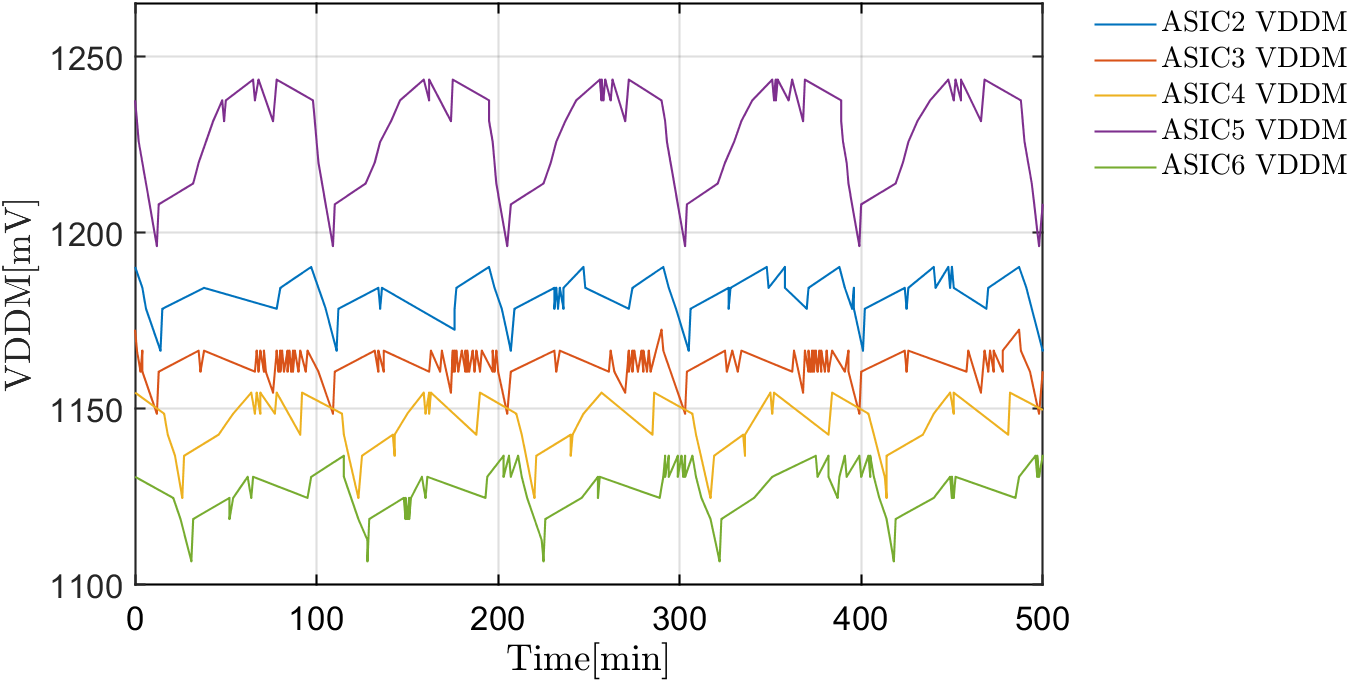
\includegraphics[width=0.75\columnwidth]{Chapter4/images/vddm_comp.png}
\caption{VDDM values comparison for different chips in the board. The tests in the chips were performed sequentially, therefore time shift between maxima of  can be seen.}
\label{feb_vary}
\end{figure}

%\newpage
Moreover, during the active cycling, 3 DS18B20 sensors were glued on the T-shelf (see section~\ref{cycling_setup}. The sensors were glued to the T-shelf, in order to determine how the temperature changes when the final thermal interfaces are used (glue between the FEB and T-shelf and carbon composite between the T-shelf and cooling block). Figure~\ref{fig_active_sensors} depicts the difference between the temperatures measured by different sensors during cycling. 

\begin{figure}[!h]
\centering
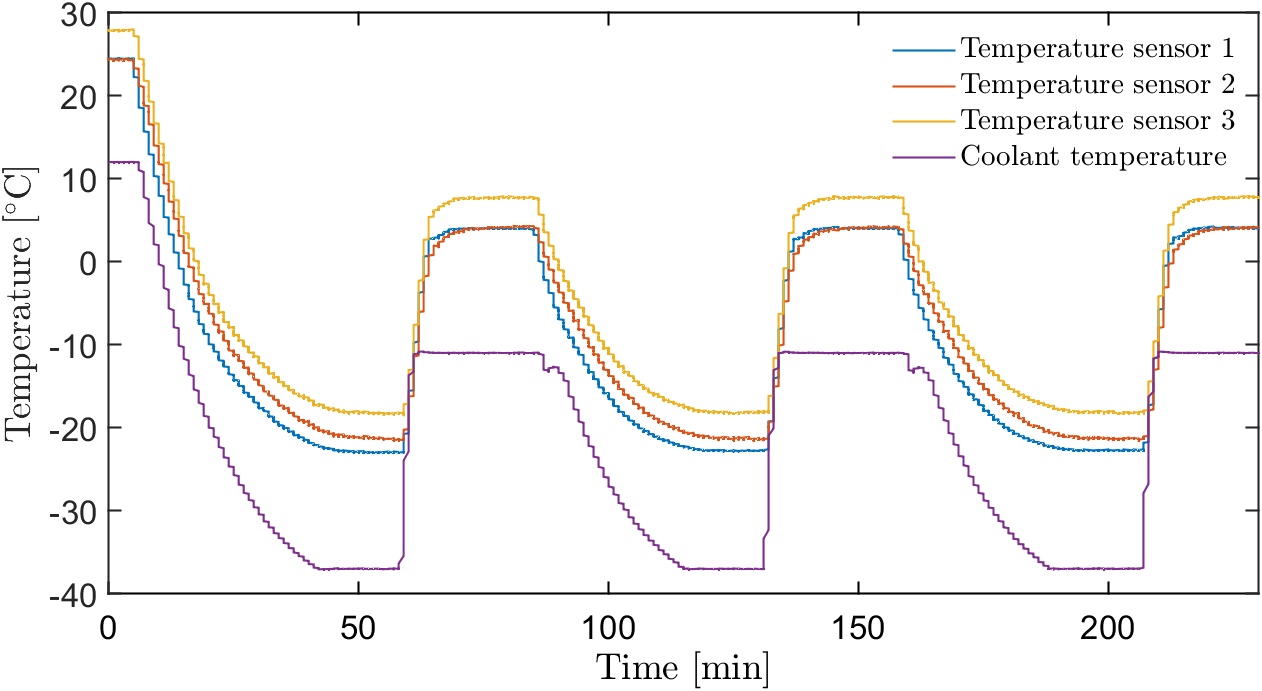
\includegraphics[width=0.75\columnwidth]{Chapter4/images/active.png}
\caption{Temperature evolution of the T-shelf during the active cycling. The DS18B20 \cite{DS18B20} sensor has an uncertainty of $\SI{0.5}{\celsius}$.}
\label{fig_active_sensors}
\end{figure}

\newpage
Temperature sensor 1 was placed above the \gls{LDO} regulators, therefore the measured values are always higher than for the two other sensors. Temperature sensor 2 was placed on top of the T-shelf but on the other side of the board. Sensor 3 was placed on the side of the T-shelf next to the powering services, its temperature is significantly lower, what is clearly visible at \SI{-38}{\celsius}, as it is placed closer to the heat exchanger (the cooling plate). This behavior was also confirmed by the simulations - see Figure~\ref{fig_nominal_febs} and Figure~\ref{fig_reboot_FEB}. 


%\newpage

\subsubsection{Low-temperature power cycling}
On contrary to the two introduced thermal cycling methods, power cycling is performed at a stable temperature. After switching the power on at low temperature, the \glspl{FEB} functionalities are tested and the power supply output is switched off. This process is then repeated a few hundred times. 

Power cycling at low temperatures is considered as one of the riskiest events that may cause a board to fail.  As identified during the irradiation of the power supplies, we should expect at least 180 radiation-induced soft errors in the low-voltage modules. Radiation-induced phenomena (latchup in the chips, and soft errors in the powering units) limit the lifetime of the electronics and could cause the boards to fail over time. \glspl{FEB} will also be power cycled during testing, commissioning, and operation of the detector, increasing the total number of power cycles up to two/three times. The previously introduced \glspl{FEB} underwent the following power cycling in low temperatures:
\begin{itemize}
    \item set A - 4 \glspl{FEB} - 200 cycles at $T = \SI{-30}{\celsius}$, 4 other \glspl{FEB} (including the one without chips) 300 cycles at $T = \SI{-30}{\celsius}$,
    \item Set B - 2 \glspl{FEB} - 50 cycles at $T = \SI{-20}{\celsius}$, 2 other \glspl{FEB} 50 cycles at $T = \SI{-30}{\celsius}$.
\end{itemize}
Figure~\ref{fig_power_cycle} shows how the current drawn by the 1.2~V \gls{LDO} regulators and 1.8~V \gls{LDO} regulators changes in the course of different tests performed in the STS-XYTERs. The highest current values (for the 1.2\,V LDO regulator) are reached during write/read tests of the registers. The changes of the 1.2\,V LDO regulator current are related to the changes of the \gls{CSA} values during testing. During one run of the testing script, the \gls{CSA} changes from 5 to 31 (the most probable range for the chip during STS operation). 
\begin{figure}[!h]
\centering
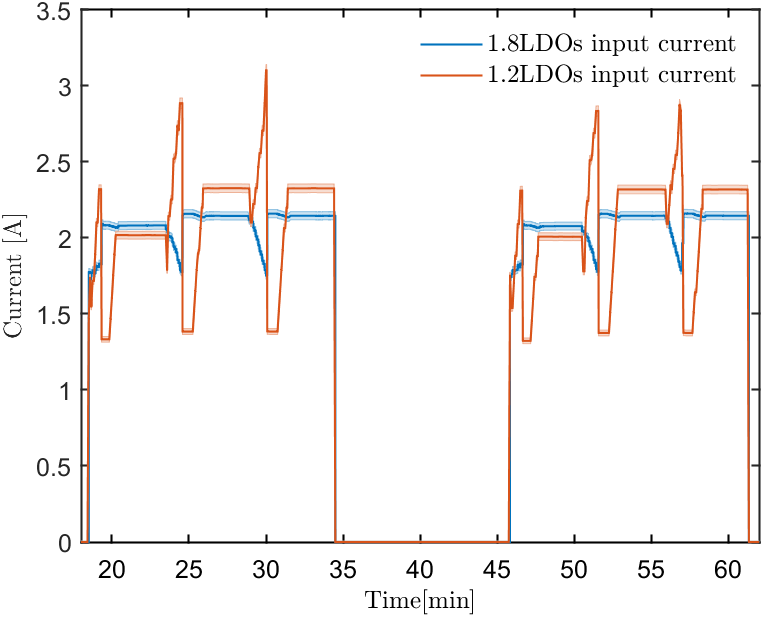
\includegraphics[width=0.6\columnwidth]{Chapter4/images/currents.png}
\caption{Cold startup of one of the \gls{FEB}: current consumed by the 1.8~V and 1.2~V \gls{LDO} regulators during the test procedure. During the period, in which the power is on, each chip undergoes 3 testing cycles.}
\label{fig_power_cycle}
\end{figure}
\subsection{Results and onset of failure analysis}
Already during preliminary thermal cycling activities (not discussed in this thesis), it was determined that the \glspl{LDO} are more prone to fail than the STS-XYTERs. Therefore, the main effort was put to gain statistics by testing multiple boards and to identify the onset of a potential \gls{LDO} regulator-related failure. To get a better understanding of the conditions leading to failures, the two sets (A and B) of measurements were compared. 


In the case of set A, which featured 8 \glspl{FEB}: 4 \glspl{FEB} with DYMAX 9001, 2 \glspl{FEB} with DYMAX 9008 as the DAM and 9001 as the fill, and 2 \glspl{FEB} without STS-XYTERs and globtop over the \gls{LDO} regulators, during the passive cycling and active cycling no failure was observed. No deterioration was observed under the microscope. First failures were detected during the power cycling at $T=\SI{-30}{\celsius}$, as summarized in Table~\ref{tab:SetA}. 

\begin{table}[!h]
\centering
\caption{Detailed description of the \gls{LDO} failure with regard to the type and number of cycles.}
\resizebox{\textwidth}{!}{%
\begin{tabular}{lll}
Globtop                   & Failure Appearence             & Remarks                       \\ \hline
DYMAX Dam 9008, fill 9001 & $\approx$ 100 power cycles     & 1.8\,V \gls{LDO} failure (AVVD18)      \\ \hline
DYMAX 9001                & $\approx$ 200 power cycles     & 1.2\,V \gls{LDO} failure after cycling  \\ \hline
DYMAX 9001                & $\approx$ 200/300 power cycles & 1.2\,V \gls{LDO} failure during cycling \\ \hline
\end{tabular}%
}
\label{tab:SetA}
\end{table}
The onset of the \gls{LDO} failure can be seen in Figure \ref{fig_cold_startup}. At about \SI{500}{\minute} the 1.2\,V LDO regulator input current started dropping, indicating increasing resistance in the circuit. As depicted in Figure \ref{fig_cold_startup} once the temperature reached $\SI{20}{\celsius}$ the current consumption was again nominal. After about  3000\,min, this effect turned out to be irreversible, and we observed the complete failure of the 1.2\,V \gls{LDO} regulator. After about 100 cycles, the current consumption measured at the level of the power supply dropped to almost 0\,A. 
%\newpage
\begin{figure}[!h]
\centering
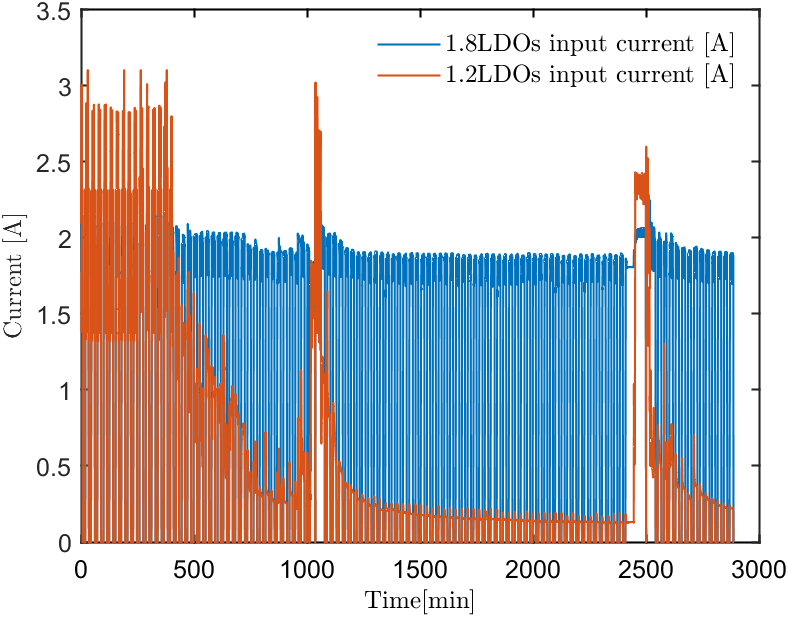
\includegraphics[width=0.46\columnwidth]{Chapter4/images/currents_long.png}
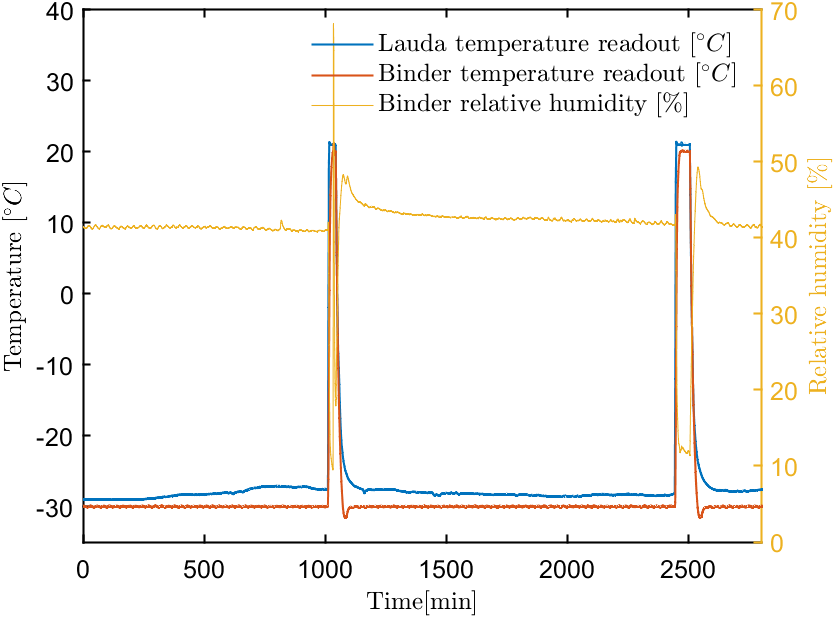
\includegraphics[width=0.48\columnwidth]{Chapter4/images/cycling.png}
\caption{Current consumed by the 1.8\,V and 1.2\,V \gls{LDO} regulators during the cold startup testing at $T = \SI{-30}{\celsius}$ (left)
Comparison of the lauda chiller setpoint, readouts from the internal temperature and relative humidity sensors of the climatic chamber (right).}
\label{fig_cold_startup}
\end{figure}

Similarly, the onset of the \gls{FEB} malfunction can be seen in the diagnostic circuit of the STS-XYTER (see figure \ref{fig_active_failure}). VDDM drops significantly, at the point at which the \gls{LDO} stops providing the nominal current. The temperature measured by the chip drops by $\SI{15}{\celsius}$, and the VDDM reaches 0\,mV, indicating a problem with 1.2\,V \gls{LDO} regulator It was later identified that one of the bond connections of the \glspl{LDO} pad got detached from the board due
to thermal stress. Therefore, the output current of the \gls{LDO} was reduced to a few mA and the voltage was not delivered to the Analog Frond End of the \glspl{ASIC}. 

% Please add the following required packages to your document preamble:
% \usepackage{graphicx}
\begin{table}[!h]
\centering
\caption{Detailed description of the \gls{LDO} failure with regard to the type and number of cycles}
\label{tab:setB}
\resizebox{\textwidth}{!}{%
\begin{tabular}{llll}
\textbf{Globtop} & Cycles                                                                                                                                                                                                                                                                                  & Failure                                                                                                     & Remarks                                                                                              \\ \hline
DYMAX 9001       & \begin{tabular}[c]{@{}l@{}}50 passive cycles {[}$\SI{-20}{\celsius}, \SI{20}{\celsius}${]}\\ 50 active cycles {[}$\SI{-20}{\celsius}, \SI{20}{\celsius}${]}\\ 50 cold startups at $T=\SI{-20}{\celsius}$\end{tabular}                                                                   & \begin{tabular}[c]{@{}l@{}}43th active cycle \\ {[}$\SI{-30}{\celsius}, \SI{-20}{\celsius}${]}\end{tabular} & 1.2\,V \gls{LDO} failure                                                                             \\ \hline
DYMAX 9001       & \begin{tabular}[c]{@{}l@{}}50 passive cycles {[}$\SI{-20}{\celsius},\SI{20}{\celsius}${]}\\ 50 active cycles {[}$\SI{-20}{\celsius}, \SI{20}{\celsius}${]}\\ 50 cold startups at $T=\SI{-20}{\celsius}$, \\ 50 active cycles {[}$\SI{-30}{\celsius}, \SI{20}{\celsius}${]}\end{tabular} & \begin{tabular}[c]{@{}l@{}}40th cold startup at \\ $T=\SI{-30}{\celsius}$\end{tabular}                      & \begin{tabular}[c]{@{}l@{}}failure of both 1.2\,V \gls{LDO}s\\ 1.8\,V \gls{LDO} failure\end{tabular} \\ \hline
DYMAX 9001       & \begin{tabular}[c]{@{}l@{}}50 passive cycles {[}$\SI{-30}{\celsius}, \SI{20}{\celsius}${]}\\ 50 active cycles {[}$\SI{-30}{\celsius}, \SI{20}{\celsius}${]}\end{tabular}                                                                                                                & \begin{tabular}[c]{@{}l@{}}29th cold startup \\ {$\SI{-40}{\celsius}$}\end{tabular}                         & 1.2\,V \gls{LDO} failure                                                                             \\ \hline
\end{tabular}%
}
\end{table}
%\newpage


\begin{figure}[!h]
\centering
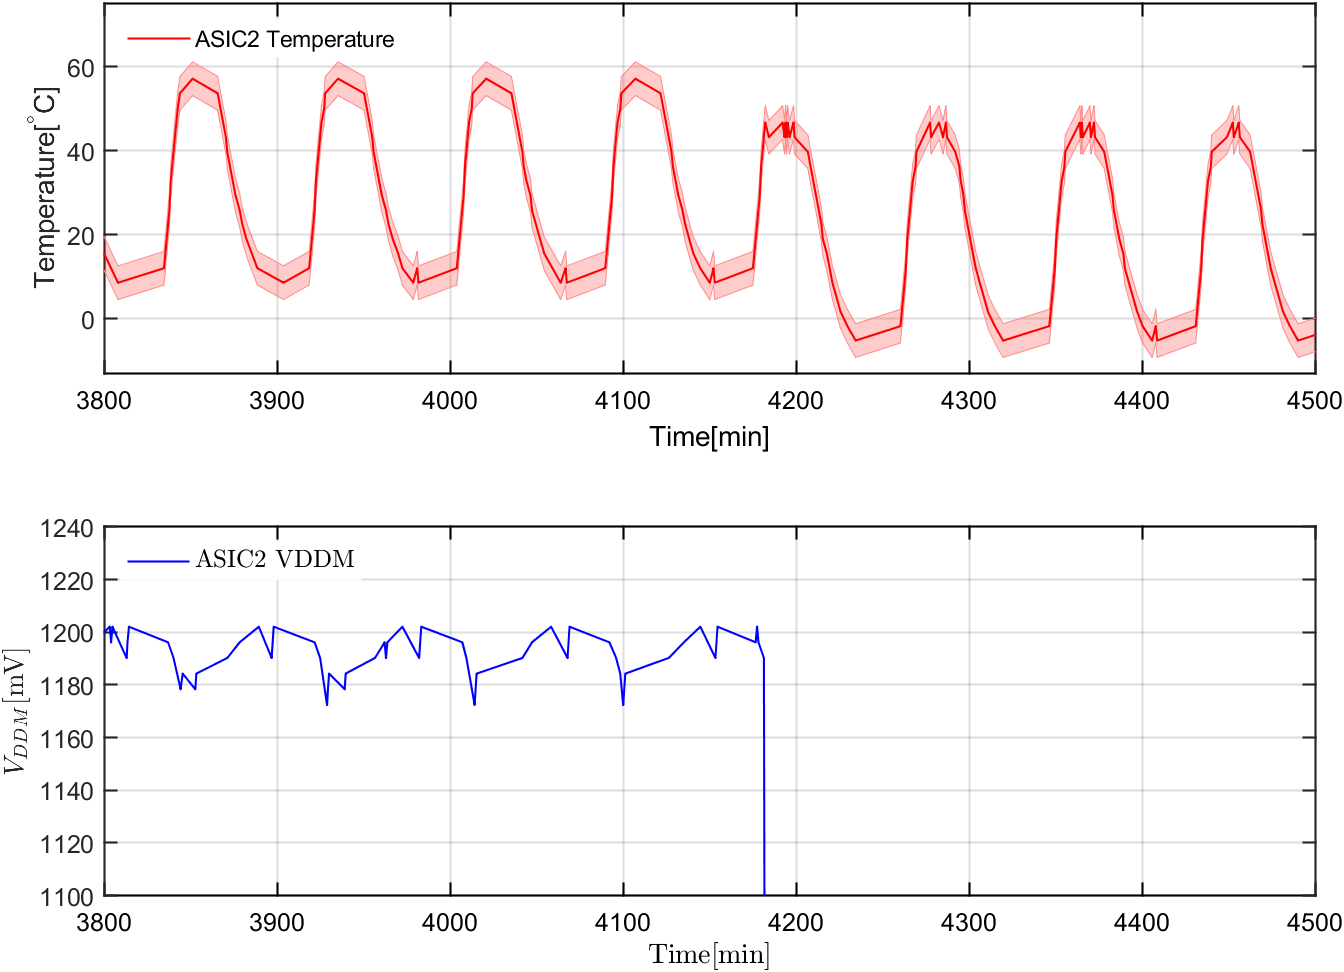
\includegraphics[width=0.6\columnwidth]{Chapter4/images/FEB2ASIC2COMP1.png}
\caption{Temperature and VDDM of a chosen STS-XYTER, and the onset of \gls{LDO} regulator failure.}
\label{fig_active_failure}
\end{figure}

One of the potential failure mechanisms can be seen in Figure~\ref{fig_ldo_lift}. An air bubble seen on the right photo caused the regulator to lift from the \glspl{PCB} surface, resulting in bond breaks. Hence, the \gls{LDO} was not providing the nominal voltage and current to the chips. 

\begin{figure}[!h]
\centering
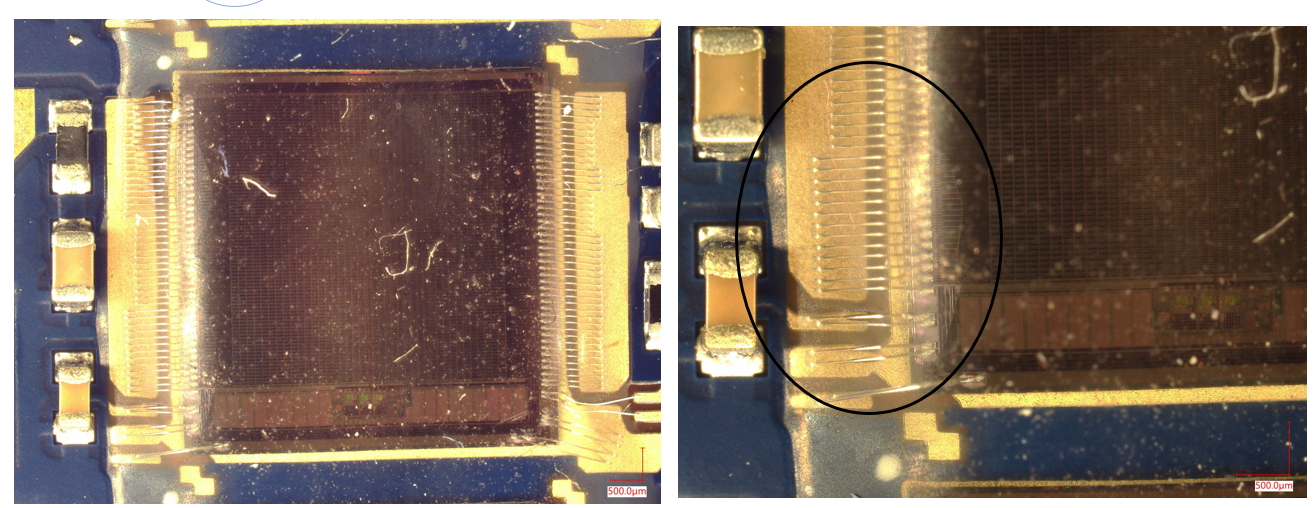
\includegraphics[width=0.8\columnwidth]{Chapter4/images/FEB_81_LDO_lift.png}
\caption{Microscopic view of the air bubble between glob top and bonds of the \gls{LDO}.}
\label{fig_ldo_lift}
\end{figure}
%\newpage
\subsection{Conclusions}
The deployed part of the developed EPICS-based framework for the thermal cycling of the \gls{STS} electronics enabled automation of the cycling process, storing the necessary data and analyzing it in order to evaluate the capabilities of the \glspl{FEB}. 

In total 12 \glspl{FEB} were investigated in order to find the safe temperature operation range. Performed thermal investigations led to discovering the limits of the \glspl{FEB}, namely failures related to the \gls{LDO} regulators. The realized measurements led to 6/24 1.2\,V \gls{LDO} failures and 2/20 1.8\,V \gls{LDO} regulator-related failures. The more frequent 1.2\,V \gls{LDO} regulator failure can be associated with larger current changes, leading to larger temperature differences. Furthermore, the boards initially tested in harsher conditions (bigger difference between the extreme temperatures) tend to fail sooner. Moreover, the \glspl{FEB} without \glspl{ASIC} and globtop on the LDO regulator didn’t show any sign of malfunction. Nevertheless, due to the lack of \glspl{ASIC}, it was impossible to change the analog line current.

As described in the introduction to thermal cycling, one of the most probable mechanisms leading to the \gls{LDO} regulator-related failure is the mismatch of the \gls{CTE}. It may potentially result in failure of the \gls{LDO} regulator due to e.g., the lift of bonds.

Findings in this section obtained through the deployed control system architecture provide crucial information on how to improve the module and their performance before the mass production of the modules for the final \gls{STS}. 

%\begin{figure}[!h]
%\centering
%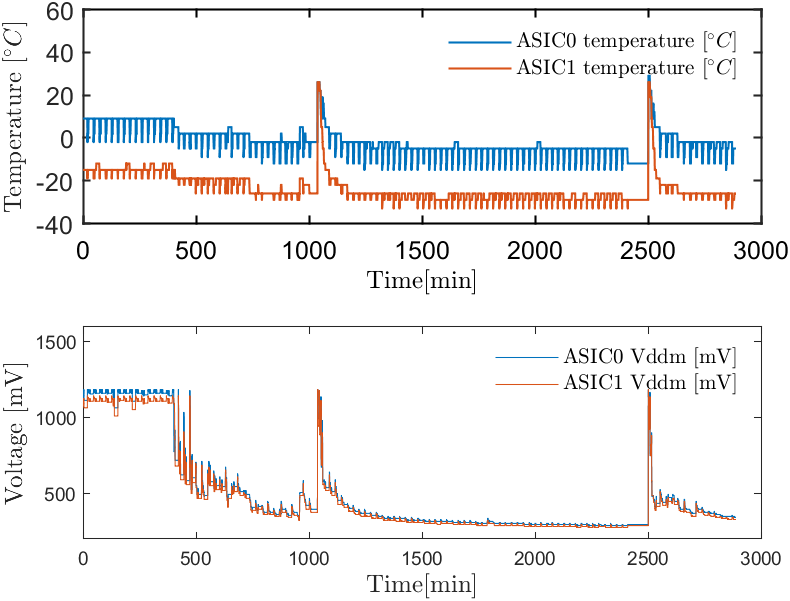
\includegraphics[width=0.6\columnwidth]{Chapter4/images/temps.png}
%\caption{A power cycle}
%\label{fig_cold_startup}
%\end{figure}

%\begin{figure}[!h]
%\centering
%\includegraphics[width=0.6\columnwidth]%{Chapter4/images/csa.png}
%\caption{A power cycle}
%\label{fig_cold_startup}
%\end{figure}

\newpage